\label{gaps} 

%\footnote{While there is a contentious debate as to whether devoicing in German is completely neutralizing \citep[e.g.,][]{Fourakis1984} or not \citep[e.g.,][]{Port1985}, it is not strictly relevant to the discussion at hand.} 

Since at least \citet{Pike1947b}, linguists have posited language-specific constraints on the contents of underlying representations.
These \emph{morpheme structure constraints} were at one time thought to fully account for speakers' knowledge of possible and impossible words (e.g., \citealt{Chomsky1965}, \citeyear[382]{SPE}, \citealt[22f.]{SPR}, \citeyear{Halle1962}, \citealt{Stanley1967}). 
\citet{Shibatani1973}, however, argues that morpheme structure constraints cannot account for all wordlikeness constraints.
In German, for instance, final obstruents devoice, and as a result, there are pairs such  [ɡʀaːt]-[ɡʀaːtə] `ridge(s)' and [ɡʀaːt]-[ɡʀaːdə] `degree(s)' differing only in the plural shape of the root.
Since the voicing of final obstruents is contrastive, the restriction on the voicing of obstruents cannot be a morpheme structure constraint. 
Yet, \citeauthor{Shibatani1973} claims that native speakers reject nonce words ending in final voiced obstruents ``\emph{on the ground that they end in voiced obstruents}'' (95). 
Thus, not all constrasts in possible wordhood can be stated as morpheme structure constraints.

Whereas \citeauthor{Shibatani1973} maintains that morpheme structure constraints are insufficient to account for speakers' knowledge of possible wordhood, others argue that morpheme structure constraints are also unnecessary. \citet[297]{Hale1965}, \citet{Kisseberth1970b}, and \citet[212f.]{Postal1968} observe that the structural descriptions of phonological processes often are often reflected in the lexical redundancies in the same language. In Russian, there are alternations implicating a process of obstruent voice assimilation, and tautomorphemic obstruent clusters have uniform voicing \citep[283]{A74}. \citet[205f.]{Dell1973} and \citet[28f.]{Stampe1973} argue that morpheme structure constraints are otiose, as phonological rules triggering alternations impose restrictions on the contents of URs, an effect known as \emph{Stampean occultation}.

There are some apparent constraints on URs which are not reflected in the system of alternations; these generalizations seem to require reference to the units of prosody (\citealt{Hooper1973}, \citealt{Kahn1976}; see \citealt{Blevins2003} and \citealt{Steriade1999} for possible alternatives). Since word-level prosodic structure is generally thought to be largely redundant and thus absent from underlying representations, these cannot be equated with morpheme structure constraints either. \citeauthor{Haugen1956} notes, for instance, that word-medial consonant cluster inventory is not arbitrary in prosodic terms.

\begin{example}[\textsc{Medial Cluster Law} (after \citealt{Haugen1956})]
\label{mcl}
A word-medial consonant cluster consists of at most a well-formed medial coda followed by a well-formed medial onset
\end{example}

Reviewing the inventory of word-medial consonant clusters in English, 
\citet{Pierrehumbert1994} notes that the vast majority of ``possible clusters'', those which can be parsed into a coda and onset, are unattested. \citeauthor{Pierrehumbert1994} argues that the cluster inventory is further filtered by what are essentially morpheme structure constraints: static co-occurrence restrictions with no support from either prosody or the system of alternations. This study will argue, however, that the only structural constraints on word-medial clusters in English are the \textsc{Medial Cluster Law} and Stampean occultation. Consequently, this domain provides no evidence for the existence of morpheme structure constraints.

\section{English syllable contact clusters \citep{Pierrehumbert1994}}

English admits a variety of word-medial consonant clusters spanning syllable boundaries which are also known as \emph{syllable contact clusters} or \emph{interludes}. These clusters can be as short as two consonants, as in \emph{a}[n.t]\emph{ics}, or as long as four, as in \emph{mi}[n.str]\emph{el}. 
There are three 

\subsection{The role of Stampean occultation}

Finally, \citeauthor{Pierrehumbert1994} does not fully consider the possible effects of Stampean occultation, as some of the static constraints she proposes may be related to English morphophonemics. For instance, she writes that ``nasal-stop sequences agree in labiality'' (175), and attributes this the status of a static constraint. However, this generalization is just a narrower form of the one derived by \textsc{Nasal Place Assimilation} (see \S\ref{npa}), and which requires no further explanation. Other derived constraints go unnoticed: for instance, she does not discuss the highly reliable tendency of obstruent-obstruent clusters to agree in voicing (see \S\ref{ova}). The evaluation below considers the role of both types of constraints on the English lexicon on an equal footing.

\subsection{The role of sparsity}

\citet{Pierrehumbert1994} infers static constraints from near-exceptionless gaps in the lexicon, but little effort is made to show that the patterns of lexical underrepresentation from which the static constraints are inferred are not due to chance. This admits the possibility that the gaps in the consonant cluster inventory are accidental rather than structural in nature \citep{Fischer-Jorgensen1952,Vogt1954}. This is made all the more likely given the tendency of segment and cluster frequency distributions to be highly skewed \citep[e.g.,][]{Pande2010,Sigurd1968,Tambovtsev2007,Weiss1961}. In Figure \ref{cao}, the rank and type frequency (i.e., frequency in the lexicon) frequency of medial codas and onsets in the lexical sample described below are graphed in log-log space. Both codas and onsets show a linear relationship between log rank and log frequency characteristic of Zipfian distributions (see Appendix \ref{zr}). As a result, an enormous lexical sample would be needed to realize clusters consistent with the \textsc{Medial Cluster Law} even if there were no constraints on the combination of medial codas and onsets in English.

\begin{figure}
\centering
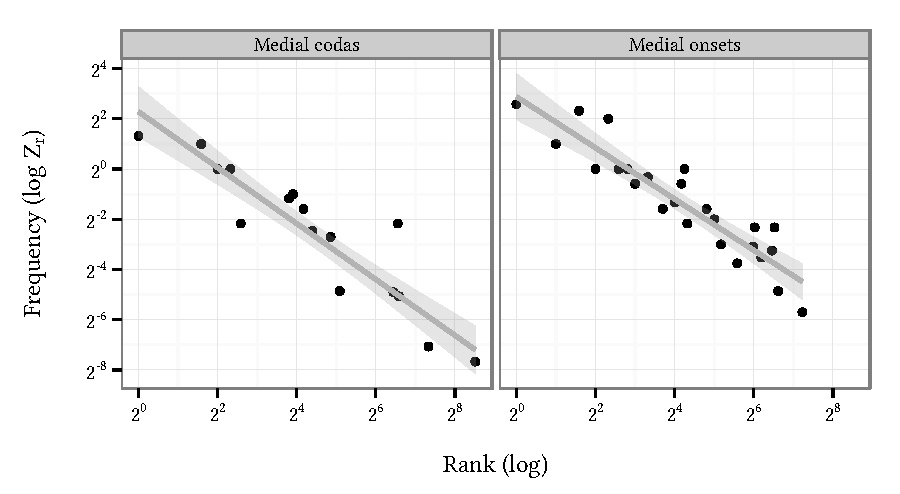
\includegraphics{co.pdf}
\caption{Medial coda and onset type frequencies in the lexical sample show a Zipfian distribution; frequencies have been smoothed using the $Z_r$ transform (see Appendix \ref{zr}).}
\label{cao}
\end{figure}

\subsection{The role of morphological segmentation}

Many components of \citeauthor{Pierrehumbert1994}'s study cannot be directly replicated. \citeauthor{Pierrehumbert1994} focuses her attention on those words she judges to be ``morphologically simple'' and ``reasonably familiar''. Since this list has neither been published nor circulated, any replication will have to be indirect. Further, it is not clear that the judgements (as well as cognitive limitations) of concerned parties should be granted evidential status in the first place, given the potential for implicit bias. A sequence which is rare in simplex words is sometimes said to mark a juncture even in the absense of other evidence for segmentation; for instance, \citet[546]{Rice2009d} analyses many words in Slave as compounds simply because they contain consonant clusters that rarely occur morph-internally. There is some evidence that infants \citep{Mattys2001b} and adults \citep{Brown1956,Hay2004a,McQueen1998b,Norris1997} use this heuristic to segment fluent speech in experimental settings. Applied indiscriminately, though, such a heuristic has the possibility to trivializes both morphological segmentation and phonotactic generalization. 

\section{Evaluation}
\label{4evaluation}

\citeauthor{Pierrehumbert1994} focuses only on triconsonantal clusters, and no reason is given for the exclusion of other sizes of clusters.

\subsection{Method}

%The same practice is sometimes applied to preserve phonological generalizations; for instance, otherwise unmotivated morphological boundaries are used in \emph{SPE} to simplify principles of stress assignment. 
Such reasoning is found in \citeauthor{Pierrehumbert1994}'s discussion of the word \emph{a}[nt.l]\emph{er}, however: this contains a cluster which violates her constraint on coda coronal obstruents, and therefore must be a complex word, she argues (see \citealt[164]{Borowsky1989} for additional exceptions to this generalization).

\subsubsection{Materials and procedure}

Following \citet[ chap.~8]{Duanmu2009} and \citet[ chap.~3]{Hammond1999a}, 
a wordlist was produced using the English portion of the CELEX database \citep{CELEX}. Any words which were coded as borrowings were excluded, as were all words not coded as ``monomorphemic''. The use of this stringent criterion eliminates many of the exceptions noted by \citeauthor{Duanmu2009} or \citeauthor{Hammond1999a} in their studies. For instance, many of the exceptions to \textsc{Obstruent Voice Assimilation} (see \S? below) noted by \citet[74]{Hammond1999a} are coded either as loanwords (e.g., \emph{vodka}, \emph{smorgasbord}) or as complex words (e.g., \emph{jurisdiction}, \emph{madcap} \emph{tadpole}, \emph{scapegoat}, \emph{magpie}). 

Unlike prior studies, ``neo-classical compounds'', words which appear to consist of a Latinate prefix and a bound stem (e.g., \emph{inspect}, \emph{excrete}) are also excluded from this wordlist. This is done in response to converging evidence that English speakers regard such words as complex. 

The treatment of Latinate forms in \emph{The sound pattern of English} (\citealt{SPE}, henceforth \emph{SPE}) assumes a prefix/bound stem decomposition. In a similar vein, \citet[11f.]{Aronoff1976} observes that Latinate forms which share the same bound stem also share irregular allomorphs of that stem under derivation. 

\begin{example}[Bound stem-specific allomorphy]
\begin{tabular}{l l l l l l}
a. & {adhere}   & {adhesion}   \\
   & {cohere}   & {cohesion}   \\
b. & {conceive} & {conception} \\
   & {perceive} & {perception} \\
\end{tabular}
\end{example}

\noindent
\citeauthor{Aronoff1976} takes this to be evidence that \emph{adhere} and \emph{cohere}, for instance, share a bound stem.

There is also a syntactic interaction between Latinate prefixes on verbs and the makeup of the verbal complement. \citet{Harley2009} observes that Latinate verbs do not generally participate in ditransitive, verb participle, or adjectival resultative constructions, all acceptable with similar Anglo-Saxon verbs \citep[see also][]{Gropen1989,Coppock2008}. 

\begin{example}[Latinate verbs and small clauses] 
\label{harley}
\begin{tabular}{l l l l@{} l}
a. & {show him the painting} & \alt{} & * & {exhibit him the painting} \\
b. & {drink himself stupid}  & \alt{} & * & {imbibe himself stupid}    \\
c. & {show it off}           & \alt{} & * & {exhibit it off}           \\
\end{tabular}
\end{example}

Results from lexical decision experiments also suggest that neoclassical compounds are complex. \citet{Taft1975,Taft1976} and \citet{Taft1986} find that nonce words like \emph{*re-sert}, which appear to be composed of a prefix and a bound stem, take longer to reject that non-words which lack apparent morphological structure such as *\emph{refant}). Bound stems also show frequency effects which are independent of their whole word frequency \citep{Taft1979,Taft2006}. Finally, \citet{Emmorey1989} and \citet{Forster2000} report facilitative priming between pairs like \emph{permit}-\emph{submit}, an effect thought to indicate of morphological relatedness.

\subsection{Results}

This filtering results in a list of 6,619 simplex words. The CELEX transcriptions of these words were then syllabified and phonologized using a technique described in Appendix \ref{syllabification}. This produces 23 unique medial codas and 40 unique medial onsets. Of the 920 ($= 21 \times 40$) medial clusters that would result from free combination, 174 (19\%) are attested. The full set of clusters and their frequencies are reproduced in Appendix \ref{clusters}. 

\subsubsection{Static constraints}

So as to account for the 81\% of ``possible'' but unattested clusters, \citet{Pierrehumbert1994} proposes three constraints on English medial clusters. These constraints are ``static'' in the sense that they have no analogues in the morphophonemics of English. 

\paragraph{Dorsal-labial clusters} \citet[173]{Pierrehumbert1994} writes that ``velar obstruents occurred only before coronals in the clusters studied, never before labials or other velars'', noting that velar-velar clusters are independently excluded by constraints on geminates (see \S?). Two-consonant velar-labial clusters are found in words like \emph{a}[k.m]\emph{e}, \emph{ru}[ɡ.b]\emph{y}, or \emph{pi}[ɡ.m]\emph{ent} occur. Table \ref{dltab} shows that velar-labial clusters are somewhat less likely to occur than  are velar-coronal clusters (e.g., \emph{ve}[k.t]\emph{or}), but such underrepresentation is not unlikely to occur by chance.

\begin{table}
\centering
\begin{tabular}{l rrrr}
\toprule
           & attested & unattested & saturation & $p$-value \\
\midrule
conforming & 25       & 91         & 22\%       & \multirow{2}{*}{0.106} \\
violating  &  4       & 40         &  9\%       \\
\bottomrule
\end{tabular}
\caption{Dorsal-labial cluster attestation in the lexical sample}
\label{dltab}
\end{table}

\paragraph{Coronal obstruent codas} \citet[175]{Pierrehumbert1994} claims that ``clusters with a coronal obstruent in the coda do not occur'', while noting exceptions like \emph{a}[nt.l]\emph{er}, \emph{ke}[s.tr]\emph{el} and \emph{oi}[nt.m]\emph{ent}. Table \ref{cctab} reveals that coda coronal obstruent clusters are not significantly less likely to occur than non-coronal obstruent clusters (e.g., \emph{re}[p.t]\emph{ile}). Restricting attention to triconsonantal clusters does not produce a significant lexical effect, either ($p = 0.129$).

\begin{table}
\centering
\begin{tabular}{l rrrr}
\toprule
           & attested & unattested & saturation & $p$-value \\
\midrule
conforming & 56       & 304        & 15\%       & \multirow{2}{*}{0.430} \\
violating  & 37       & 243        & 13\%       \\
\bottomrule
\end{tabular}
\caption{Coda coronal obstruent cluster attestation in the lexical sample}
\label{cctab}
\end{table}

\paragraph{ABA clusters} \citet[][176]{Pierrehumbert1994} notes the ``lack of clusters with identical first and third elements'', ignoring presence or absence of voicing. Despite the fact that the corpus contains no exceptions to this generalization, these \textsc{ABA} clusters are not significantly less common than other triconsonantal and quadraconsonantal clusters (Table \ref{abatab}).

\begin{table}
\centering
\begin{tabular}{l rrrr}
\toprule
           & attested & unattested & saturation & $p$-value \\
\midrule
conforming & 47       & 512        &  8\%       & \multirow{2}{*}{0.250} \\
violating  &  0       &  25        &  0\%       \\
\bottomrule
\end{tabular}
\caption{ABA cluster attestation in the lexical sample}
\label{abatab}
\end{table}

\paragraph{Summary} There is no statistical support for \citeauthor{Pierrehumbert1994}'s static constraints.

\subsubsection{Derived constraints}

FIXME

\paragraph{Obstruent voice assimilation}
\label{ova}

Voice assimilation alternations are evidenced by the non-syllabic allomorphs of the regular past (e.g., \emph{nap}[t] $\sim$ \emph{nab}[d]) and noun plural (e.g., \emph{lap}[s] $\sim$ \emph{lab}[z]), which take the voicing specification of a preceding obstruent.\footnote{Underlying /-d, -z/ are assumed here (e.g., \citealt{Anderson1973a}, \citealt[284f.]{Bakovic2005b}, \citealt{Basboll1972}, \citealt[210]{SPE}, \citealt[282]{Hockett1958}, \citealt[102]{Pinker1988}, \citealt{Shibatani1972}); alternative analyses are put forth by \citet[210f.]{LANGUAGE}, \citet[135]{Borowsky1986}, \citet{Hoard1971}, \citet{Kiparsky1985}, \citet{Lightner1970}, \citet{Luelsdorff1969}, \citet{Miner1975}, \citet[426]{Nida1948}, and \citet{Zwicky1975}.}
%Bizarely, \citet[208]{Wetzels2001}, cite English as an example of a language without ``general devoicing or assimilatory effects''. 

\begin{example}[\textsc{Obstruent Voice Assimilation}]
\label{ovarule}
$\begin{bmatrix} -\textsc{Son} \end{bmatrix}~\goesto~\begin{bmatrix} =\textsc{Voi} \end{bmatrix}~/~\gap~\begin{bmatrix} =\textsc{Voi} \\ -\textsc{Son} \end{bmatrix}$
\end{example}

\noindent
\citet{Pierrehumbert1994} does not discuss a constraint against adjacent obstruents disagreeing in voice. As shown in Table \ref{ovatab} however, the vast majority of medial obstruents clusters in simplex words are either uniformly voiced, as in \emph{hu}[z.b]\emph{and}, or uniformly voiceless, as in or \emph{rha}[p.s]\emph{osdy}, and hetero-voiced clusters, like those in \emph{a}[b.s]\emph{inth} and \emph{a}[s.b]\emph{estos} are rarer than would be expected from chance.

\begin{table}
\centering
\begin{tabular}{l rrrr}
\toprule
           & attested & unattested & saturation & $p$-value \\
\midrule
conforming & 35       & 329        & 10\%       & \multirow{2}{*}{0.002} \\
violating  & 11       & 305        &  3\%       \\
\bottomrule
\end{tabular}
\caption{Obstruent voice assimilation cluster attestation in the lexical sample}
\label{ovatab}
\end{table}

\paragraph{Nasal place assimilation}
\label{npa}

\textsc{Nasal Place Assimilation} (e.g., \citealt[149]{Borowsky1986}, \emph{SPE}:85, \citealt[62]{Halle1985a}) accounts for [n $\sim$ ŋ] allophony as well as Latinate prefix allomorphy.

\begin{example}[\emph{im-}/\emph{in-} allomorphy]
\label{nparule}
\begin{tabular}{l l l l l l l}
a. & {polite}   & {i}[m.p]{olite}   & & {balance} & {i}[m.b]{alance} \\
b. & {tangible} & {i}[n.t]{angible} & & {decent}  & {i}[n.d]{ecent}  \\
\end{tabular}
\end{example}

%Furthermore, \citet[228]{Myers1993} reports speech errors which create nasal-obstruent clusters and undergo \textsc{Nasal Place Assimilation}; e.g., \emph{ra}[nd] \emph{orker}, intended \emph{ra}[ŋk] \emph{order}. 

\noindent
The rule is formalized below.

\begin{example}[\textsc{Nasal Place Assimilation}]
$\begin{bmatrix} $+$\textsc{Nas} \end{bmatrix}~\goesto~\begin{bmatrix} =\textsc{Lab} \\ =\textsc{Cor} \\ =\textsc{Dor} \end{bmatrix}~/~\gap{}~\begin{bmatrix} =\textsc{Lab} \\ =\textsc{Cor} \\ =\textsc{Dor} \\ -\textsc{Son} \end{bmatrix}$
\end{example}

As shown in Table \ref{npatab}, virtually all (94\%) clusters of a nasal coda followed by a homorganic obstruent (e.g., \emph{pi}[m.p]\emph{le}, \emph{sta}[n.z]\emph{a}, \emph{mo}[ŋ.k]\emph{ey}) are attested. As \citet[175]{Pierrehumbert1994} observes, heterorganic clusters, like those \emph{pli}[m.s]\emph{oll} or \emph{scri}[m.ʃ]\emph{aw}, do occur, but they are significantly more rare.

\begin{table}
\centering
\begin{tabular}{l rrrr}
\toprule
           & attested & unattested & saturation & $p$-value \\
\midrule
conforming & 31       & 2          & 94\%       & \multirow{2}{*}{3.37\e{-07}} \\
violating  & 11       & 22         & 33\%       \\
\bottomrule
\end{tabular}
\caption{Nasal place assimilation cluster attestation in the lexical sample}
\label{npatab}
\end{table}

\paragraph{Degemination} The final alternation found in English medial clusters is the simplification of geminates which is characteristic of ``level I'' morphology, and is found in the irregular /-t/ past tense (e.g., \emph{bend}/\emph{ben}[t], \emph{build}/\emph{buil}[t]) and in \emph{-ly} deadjectival derivatives (e.g., \emph{norma}[l]\emph{y}, cf. \emph{calm}[l]\emph{y}), and Latinate prefix allomorphy (\emph{SPE}:148; \citealt[102]{Borowsky1986}). \textsc{Degemination} is formalized here as a rule deleting the first of two identical segments, ignoring voice. 

\begin{example}[\textsc{Degemination}]
$\begin{bmatrix} =\textsc{Lab} \\ =\textsc{Cor} \\ =\textsc{Dor} \\ =\textsc{Son} \\ \ldots{} \end{bmatrix}~\goesto~\emptyset~\big /~\gap~\begin{bmatrix} =\textsc{Lab} \\ =\textsc{Cor} \\ =\textsc{Dor} \\ =\textsc{Son} \\ \ldots{} \end{bmatrix}$
\end{example}

\noindent
As can be seen from Table \ref{degemtab}, the sample includes no sequences of identical segments, or of identical segments differing only in voice, something highly unlikely to arise by chance.

\begin{table}
\centering
\begin{tabular}{l rrrr}
\toprule
           & attested & unattested & saturation & $p$-value \\
\midrule
conforming & 173      & 643        & 21\%       & \multirow{2}{*}{1.2\e{-10}} \\
violating  & 0        & 104        & 0\%        \\
\bottomrule
\end{tabular}
\caption{Degemination in the lexical sample}
\label{degemtab}
\end{table}

\paragraph{Summary} All three of \emph{SPE} rules targeting medial clusters have a robust effect in constraining the inventory of possible word-medial syllable clusters; possible clusters which are surface exceptions to these three rules are much less likely to be attested than those which conform to them. 

\subsubsection{Computational models}

A soft-margin support vector machine \citep{Cortes1995} with a linear kernel is used to convert from the per-cluster scores to attestation predictions
, by finding a single cutoff which optimally separates attested and unattes
ted clusters according to their model scores. 

It is possible to maximize recall at the expense of precision, by predicting all clusters to be unattested, or to increase precision at the expense of recall, by predicting non-attestation for a great number of clusters. $F_1$, the harmonic mean of these two measures, is a balanced measure of this tradeoff.

This is not put forth as a cognitively plausible model for learning of phonotactics; it simply represents an upper bound for classifying possible clusters. 

The results for are summarized in Table \ref{cmresults}.

\paragraph{Null baseline} Since the majority of possible clusters are unattested, a null baseline which predicts all clusters to be unattested achieves classifies 81\% of clusters correctly, achieving perfect recall at the price of precision.

\paragraph{Expected frequency} \citet{Pierrehumbert1994} proposes that the well-formedness of a syllable contact clusters is proportional to the independent probability of the coda and onset that make it up. \citeauthor{Pierrehumbert1994} reports that this is the best predictor of which complex clusters occur, and while it is a significant improvement on the baseline (sign test $p = 4.5$\e{-05}), it is not distinguished in performance from the other models under consideration.

\paragraph{Derived constraints} The three derived generalizations define a simple classifier, predicting attestation for all clusters which do not violate these three generalizations. This is a significant improvement on the null baseline (sign test $p = 4.0$\e{-09}), preserving high recall while improving precision. The predictions of the derived constraints classifier can also be combined with information on expected frequency. As expected, this boosts precision, since FIXME. This combination produces a model with the highest accuracy and $F_1$.

\paragraph{Maximum entropy phonotactics} \citet{Hayes2008a} present a model which uses the principle of maximum entropy to weigh a large number of competing phonotactic constraints. Since this model has many experimenter-determined parameters, a direct replication of the experiments reported by \citealt{Hayes2008a} is attempted; their software, feature specification, and model settings are all used. Training in this model is inherently stochastic, producing slightly different constraints and weights on each run, so the least accurate of ten independent runs is used for evaluation; this is also the practice of \citeauthor{Hayes2008a}. This model performs approximately as well as other classifiers, but has the poorest recall; this suggests that the constraints learned are overly narrow and fail to filter out many impossible clusters. FIXME

\paragraph{Summary} FIXME

\begin{table} 
\centering
\begin{tabular}{l | rrrr}
\toprule
                    & accuracy & precision & recall & $F_1$ \\
\midrule
Baseline            & 0.812    & 0.812     & 1.000  & 0.896 \\
Expected frequency  & 0.836    & 0.845     & 0.984  & 0.909 \\
Derived constraints & 0.838    & 0.840     & 0.997  & 0.912 \\
DC \& EF            & 0.861    & 0.868     & 0.988  & 0.924 \\
\citet{Hayes2008a}  & 0.835    & 0.942     & 0.854  & 0.896 \\
\bottomrule
\end{tabular}
\caption{Results of the cluster classification task; a combination of derived constraints and expected frequency (``DC \& EF'') produces the highest accuracy and $F_1$.}
\label{cmresults}
\end{table}

\subsection{Discussion}

FIXME

\subsubsection{The probability of accidental gaps}

\begin{unlabeledexample}
$\displaystyle \hat{p}_0 = \frac{n_1}{N}$
\end{unlabeledexample}

%67 types occur once
%67 / 977
%7\% 

\subsubsection{Simulating medial clusters}
\label{simulate}

\begin{example}[Simulation procedure]
\begin{tabular}{l l}
a. & Sample a medial coda according to the observed probabilities  \\
b. & Sample a medial onset according to the observed probabilities \\
c. & Apply all matching \emph{SPE} rules to cluster formed by their concatenation \\
\end{tabular}
\end{example}

\begin{figure}
\centering
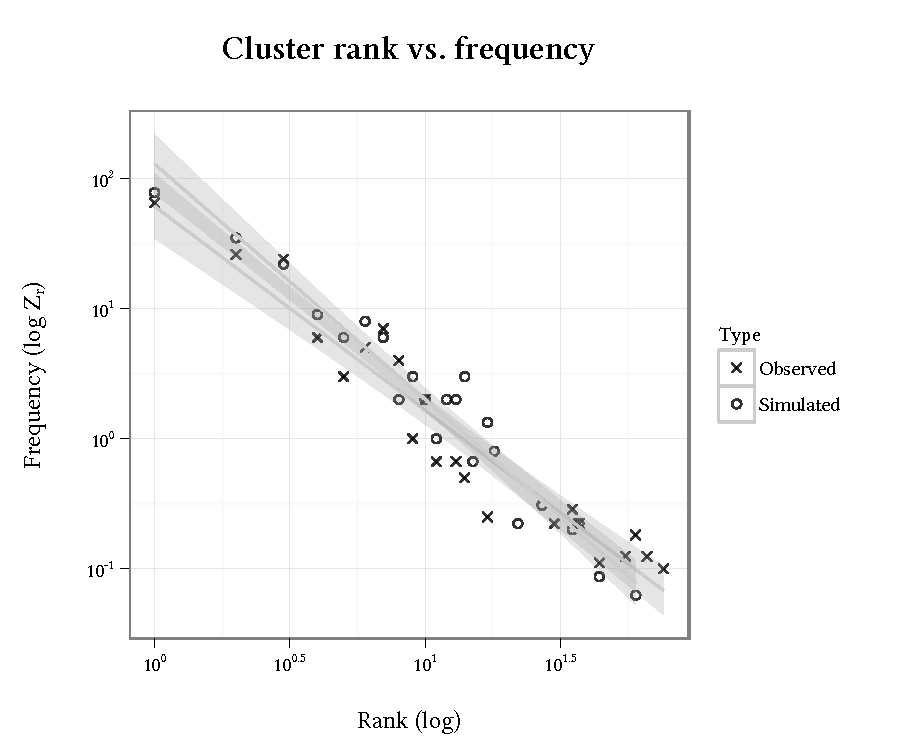
\includegraphics{sim.pdf}
\caption{A simulated cluster inventory, generated by random sampling and applying phonological neutralizations closely matches the observed cluster frequencies (represented by the smoothing line). Simulated and observed frequencies have been smoothed using the $Z_r$ transform.}
\label{sim}
\end{figure}

real ($\alpha = -1.65$, $R^2 = 0.940$)
fake ($\alpha = -1.58$, $R^2 = 0.945$)
fitt ($R^2 = 0.712$, $p = 4.5$\e{-05})

In summary, the sparse cluster inventory, previously taken as evidence for static constraints on syllable contact clusters, is expected even if the only constraints on possible clusters are those which are phonologically derived.

\section{Conclusions}

None of the foregoing results have revealed any evidence for structural constraints on the English syllable contact cluster except those derived from phonological alternations. What then is to be said of the 366 clusters which do not violate a derived constraint, but which are yet unattested, like [b.z] or [z.n]? Since these gaps appear to be quite arbitrary from a phonological perspective---they cannot be reliably discovered either by linguist or computer---it seems reasonable to identify these clusters as accidental gaps, resulting from the sparsity of the sample and of the English lexicon. 

%It is quite apparent that root-internal hetero-voiced obstruent clusters like [s.b] or [z.t] are also rare compared to clusters which are uniformly voiced or uniformly voiceless, as predicted the assimilation rule. Yet, \citet{Pierrehumbert1994} does not mention voice assimilation in her study of English syllable contact clusters. \citet[][74f.]{Hammond1999a} cites words like \emph{a}[b.s]\emph{inth} and \emph{a}[s.b]\emph{estos}, which contain hetero-voiced obstruent clusters, as evidence that the process does not apply root-internally, though few of his examples are in fact simplex according to CELEX.\footnote{The \textsc{Revised Alternation Condition} (RAC) proposed by \citeauthor{Kiparsky1973a} (\citeyear{Kiparsky1973a}:163, \citeyear{Kiparsky1982a}:152) blocks the application of obligatory neutralization processes like \textsc{Obstruent Voice Assimilation} in root-internal (i.e., non-derived) environments. Simply because there are exceptions in non-derived environments, \textsc{Obstruent Voice Assimilation} is always consistent with the RAC whether or not it actually applies in non-derived environments. This is due to the ``obligatory'' condition of the RAC. If the rule applies in non-derived environments, then it has lexical exceptions (e.g., \emph{a}[s.b]\emph{estos}) and is not obligatory and thus free from the RAC. On the other hand, if the rule is subject to the RAC, it only applies in derived environments, in which it is obligatory.}
% 
%The question is: does \textsc{Obstruent Voice Assimilation} contribute a meaningful characterization the English lexicon? More specifically, are hetero-voiced clusters underrepresented in a way that is unlikely under the hypothesis of free combination? To answer this question, the 720 clusters in which both the final coda consonant and initial onset consonant are obstruent are sorted into four bins, according to whether they are attested or not, and whether or not the conform to the derived constraint---both obstruents are either voiced or voiceless, like in \emph{hu}[z.b]\emph{and} or \emph{rha}[p.s]\emph{osdy}, respectively---or violate it, like the aforementioned \emph{a}[b.s]\emph{inth} and \emph{a}[s.b]\emph{estos}. 

%\citet{McGowan2009} claims that the type frequency of individual syllable contact clusters in English is predicted by the change of sonority in the clusters.\footnote{Thanks to Maria Gouskova for bringing this study to my attention.} Using a sonority scale proposed by \citet{Jespersen1904}, \citeauthor{McGowan2009} reports that clusters like [m.p], with sharply falling sonority, are slightly more frequent than those like [t.j], with rising sonority. However, \citeauthor{McGowan2009} finds that sonority of clusters accounts for a very small of the variance in cluster frequency ($R^2 = 0.077$). As a predictor of cluster attestation, sonority distance provided no improvement over the null baseline; consequently, it is not included in Table \ref{cmresults}.
